\documentclass[17pt,a4paper,landscape]{extarticle}
\usepackage[margin=2.35cm,top=0.12cm,left=1.05cm]{geometry}
\usepackage{amsmath}
\usepackage{amssymb}
\usepackage{tasks}
\usepackage{tikz}
\usepackage{xcolor}
\usepackage[sfdefault,lf]{FiraSans}
\renewcommand{\familydefault}{\sfdefault}
\setlength{\parindent}{0pt}
\pagestyle{empty}
\settasks{label=\textbf{\arabic*.}, label-width=2.2em, item-indent=2.95em, column-sep=2.1cm, after-item-skip=4.7em}
\renewcommand{\arraystretch}{1.15}
\everymath{\displaystyle}

\begin{document}
\sffamily
\boldmath

\boldmath

\boldmath

{\LARGE \textbf{Perimeter (shapes with straight edges only) --- Proficient}}
\begin{tasks}(3)
\task Find the perimeter.\\[0.4em]
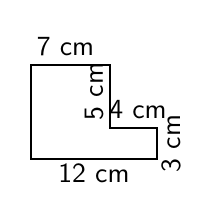
\begin{tikzpicture}[x=0.20cm,y=0.20cm,baseline=(current bounding box.center)]
  \draw[thick] (0,0)--(8,0)--(8,2)--(5,2)--(5,6)--(0,6)--cycle;
  \node at (4,-0.9) {12 cm};
  \node[rotate=90] at (8.9,1) {3 cm};
  \node at (6.8,3.2) {4 cm};
  \node[rotate=90] at (4.0,4.3) {5 cm};
  \node at (2.2,7.2) {7 cm};
\end{tikzpicture}
\task Find the perimeter.\\[0.4em]
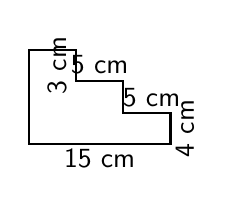
\begin{tikzpicture}[x=0.20cm,y=0.20cm,baseline=(current bounding box.center)]
  \draw[thick] (0,0)--(9,0)--(9,2)--(6,2)--(6,4)--(3,4)--(3,6)--(0,6)--cycle;
  \node at (4.5,-0.9) {15 cm};
  \node[rotate=90] at (9.9,1) {4 cm};
  \node at (7.8,3.0) {5 cm};
  \node at (4.5,5.1) {5 cm};
  \node[rotate=90] at (1.8,5) {3 cm};
\end{tikzpicture}
\task Find the perimeter.\\[0.4em]
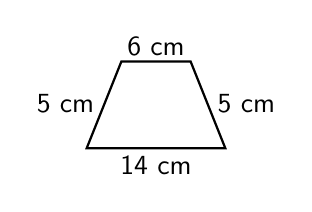
\begin{tikzpicture}[x=0.22cm,y=0.22cm,baseline=(current bounding box.center)]
  \draw[thick] (0,0)--(8,0)--(6,5)--(2,5)--cycle;
  \node at (4,-1.0) {14 cm};
  \node at (4,5.9) {6 cm};
  \node at (1.0,2.6) [left] {5 cm};
  \node at (7.0,2.6) [right] {5 cm};
\end{tikzpicture}
\task Find the perimeter.\\[0.4em]
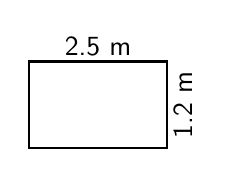
\begin{tikzpicture}[x=0.22cm,y=0.22cm,baseline=(current bounding box.center)]
  \draw[thick] (0,0) rectangle (8,5);
  \node at (4,5.9) {2.5 m};
  \node[rotate=90] at (8.9,2.5) {1.2 m};
\end{tikzpicture}
\task Find the perimeter.\\[0.4em]
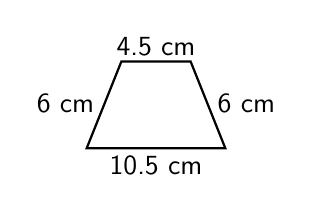
\begin{tikzpicture}[x=0.22cm,y=0.22cm,baseline=(current bounding box.center)]
  \draw[thick] (0,0)--(8,0)--(6,5)--(2,5)--cycle;
  \node at (4,-1.0) {10.5 cm};
  \node at (4,5.9) {4.5 cm};
  \node at (1.0,2.6) [left] {6 cm};
  \node at (7.0,2.6) [right] {6 cm};
\end{tikzpicture}
\task Find the perimeter.\\[0.4em]
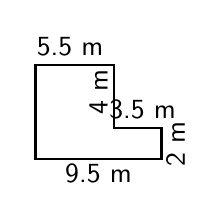
\begin{tikzpicture}[x=0.20cm,y=0.20cm,baseline=(current bounding box.center)]
  \draw[thick] (0,0)--(8,0)--(8,2)--(5,2)--(5,6)--(0,6)--cycle;
  \node at (4,-0.9) {9.5 m};
  \node[rotate=90] at (8.9,1) {2 m};
  \node at (6.8,3.2) {3.5 m};
  \node[rotate=90] at (4.0,4.3) {4 m};
  \node at (2.2,7.2) {5.5 m};
\end{tikzpicture}
\task A rectangle has perimeter 38 cm and width 7 cm. Find its length.
\task A square garden has perimeter 18 m. How long is each side?
\task A triangle has sides 7.2 cm, 5.8 cm and 6.5 cm. Find its perimeter.
\task A shape has side lengths 4 cm, 6 cm, 3 cm, 5 cm, 2 cm and 8 cm. Find its perimeter.
\task Jordan says a \mbox{$9$} cm by \mbox{$4$} cm rectangle has perimeter \mbox{$13$} cm. Explain the mistake and give the correct perimeter.
\task A rectangle is twice as long as it is wide. Its perimeter is 30 cm. Find the length and width.
\task The perimeter of an equilateral triangle is 27 cm. Find one side length.
\task A rectangle is 13 m long and 4 m wide. Find its perimeter.
\task A regular pentagon has side length 6 cm. Find its perimeter.
\task The perimeter of a square is 44 mm. Find one side length.
\end{tasks}

\end{document}
